% Created by tikzDevice version 0.12.3 on 2020-08-14 16:27:15
% !TEX encoding = UTF-8 Unicode
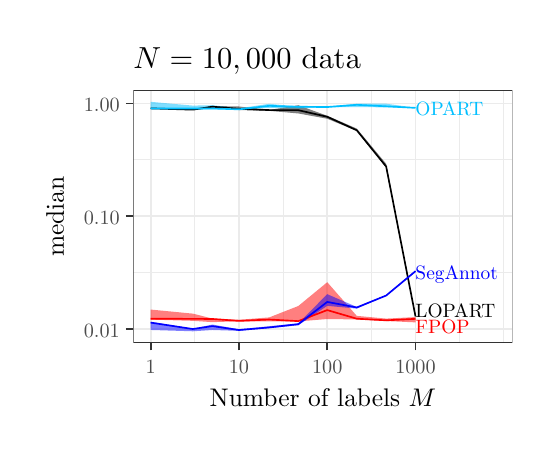
\begin{tikzpicture}[x=1pt,y=1pt]
\definecolor{fillColor}{RGB}{255,255,255}
\path[use as bounding box,fill=fillColor,fill opacity=0.00] (0,0) rectangle (180.67,144.54);
\begin{scope}
\path[clip] (  0.00,  0.00) rectangle (180.67,144.54);
\definecolor{drawColor}{RGB}{255,255,255}
\definecolor{fillColor}{RGB}{255,255,255}

\path[draw=drawColor,line width= 0.6pt,line join=round,line cap=round,fill=fillColor] (  0.00,  0.00) rectangle (180.68,144.54);
\end{scope}
\begin{scope}
\path[clip] ( 38.23, 30.69) rectangle (175.17,121.88);
\definecolor{fillColor}{RGB}{255,255,255}

\path[fill=fillColor] ( 38.23, 30.69) rectangle (175.18,121.88);
\definecolor{drawColor}{gray}{0.92}

\path[draw=drawColor,line width= 0.3pt,line join=round] ( 38.23, 56.07) --
	(175.17, 56.07);

\path[draw=drawColor,line width= 0.3pt,line join=round] ( 38.23, 96.78) --
	(175.17, 96.78);

\path[draw=drawColor,line width= 0.3pt,line join=round] ( 60.40, 30.69) --
	( 60.40,121.88);

\path[draw=drawColor,line width= 0.3pt,line join=round] ( 92.30, 30.69) --
	( 92.30,121.88);

\path[draw=drawColor,line width= 0.3pt,line join=round] (124.20, 30.69) --
	(124.20,121.88);

\path[draw=drawColor,line width= 0.3pt,line join=round] (156.09, 30.69) --
	(156.09,121.88);

\path[draw=drawColor,line width= 0.3pt,line join=round] (172.04, 30.69) --
	(172.04,121.88);

\path[draw=drawColor,line width= 0.6pt,line join=round] ( 38.23, 35.72) --
	(175.17, 35.72);

\path[draw=drawColor,line width= 0.6pt,line join=round] ( 38.23, 76.43) --
	(175.17, 76.43);

\path[draw=drawColor,line width= 0.6pt,line join=round] ( 38.23,117.13) --
	(175.17,117.13);

\path[draw=drawColor,line width= 0.6pt,line join=round] ( 44.45, 30.69) --
	( 44.45,121.88);

\path[draw=drawColor,line width= 0.6pt,line join=round] ( 76.35, 30.69) --
	( 76.35,121.88);

\path[draw=drawColor,line width= 0.6pt,line join=round] (108.25, 30.69) --
	(108.25,121.88);

\path[draw=drawColor,line width= 0.6pt,line join=round] (140.14, 30.69) --
	(140.14,121.88);
\definecolor{fillColor}{RGB}{255,0,0}

\path[fill=fillColor,fill opacity=0.50] ( 44.45, 42.68) --
	( 59.67, 41.21) --
	( 66.75, 39.43) --
	( 76.35, 38.99) --
	( 87.27, 39.84) --
	( 97.79, 43.96) --
	(108.25, 52.56) --
	(118.92, 40.40) --
	(129.54, 39.41) --
	(140.14, 39.96) --
	(140.14, 38.05) --
	(129.54, 38.54) --
	(118.92, 39.11) --
	(108.25, 39.26) --
	( 97.79, 38.40) --
	( 87.27, 38.38) --
	( 76.35, 38.45) --
	( 66.75, 38.13) --
	( 59.67, 38.61) --
	( 44.45, 39.05) --
	cycle;

\path[] ( 44.45, 42.68) --
	( 59.67, 41.21) --
	( 66.75, 39.43) --
	( 76.35, 38.99) --
	( 87.27, 39.84) --
	( 97.79, 43.96) --
	(108.25, 52.56) --
	(118.92, 40.40) --
	(129.54, 39.41) --
	(140.14, 39.96);

\path[] (140.14, 38.05) --
	(129.54, 38.54) --
	(118.92, 39.11) --
	(108.25, 39.26) --
	( 97.79, 38.40) --
	( 87.27, 38.38) --
	( 76.35, 38.45) --
	( 66.75, 38.13) --
	( 59.67, 38.61) --
	( 44.45, 39.05);
\definecolor{fillColor}{RGB}{0,0,0}

\path[fill=fillColor,fill opacity=0.50] ( 44.45,115.51) --
	( 59.67,115.10) --
	( 66.75,116.25) --
	( 76.35,116.06) --
	( 87.27,114.80) --
	( 97.79,116.51) --
	(108.25,112.71) --
	(118.92,108.07) --
	(129.54, 95.35) --
	(140.14, 40.61) --
	(140.14, 40.17) --
	(129.54, 94.06) --
	(118.92,107.22) --
	(108.25,111.63) --
	( 97.79,113.54) --
	( 87.27,114.48) --
	( 76.35,114.78) --
	( 66.75,115.68) --
	( 59.67,114.87) --
	( 44.45,115.36) --
	cycle;

\path[] ( 44.45,115.51) --
	( 59.67,115.10) --
	( 66.75,116.25) --
	( 76.35,116.06) --
	( 87.27,114.80) --
	( 97.79,116.51) --
	(108.25,112.71) --
	(118.92,108.07) --
	(129.54, 95.35) --
	(140.14, 40.61);

\path[] (140.14, 40.17) --
	(129.54, 94.06) --
	(118.92,107.22) --
	(108.25,111.63) --
	( 97.79,113.54) --
	( 87.27,114.48) --
	( 76.35,114.78) --
	( 66.75,115.68) --
	( 59.67,114.87) --
	( 44.45,115.36);
\definecolor{fillColor}{RGB}{0,191,255}

\path[fill=fillColor,fill opacity=0.50] ( 44.45,117.74) --
	( 59.67,116.38) --
	( 66.75,116.52) --
	( 76.35,115.39) --
	( 87.27,117.02) --
	( 97.79,116.01) --
	(108.25,116.01) --
	(118.92,117.08) --
	(129.54,117.07) --
	(140.14,115.59) --
	(140.14,115.53) --
	(129.54,115.74) --
	(118.92,115.86) --
	(108.25,115.82) --
	( 97.79,115.33) --
	( 87.27,115.59) --
	( 76.35,115.00) --
	( 66.75,114.99) --
	( 59.67,114.95) --
	( 44.45,115.34) --
	cycle;

\path[] ( 44.45,117.74) --
	( 59.67,116.38) --
	( 66.75,116.52) --
	( 76.35,115.39) --
	( 87.27,117.02) --
	( 97.79,116.01) --
	(108.25,116.01) --
	(118.92,117.08) --
	(129.54,117.07) --
	(140.14,115.59);

\path[] (140.14,115.53) --
	(129.54,115.74) --
	(118.92,115.86) --
	(108.25,115.82) --
	( 97.79,115.33) --
	( 87.27,115.59) --
	( 76.35,115.00) --
	( 66.75,114.99) --
	( 59.67,114.95) --
	( 44.45,115.34);
\definecolor{fillColor}{RGB}{0,0,255}

\path[fill=fillColor,fill opacity=0.50] ( 44.45, 38.29) --
	( 59.67, 35.74) --
	( 66.75, 37.26) --
	( 76.35, 35.55) --
	( 87.27, 36.65) --
	( 97.79, 37.69) --
	(108.25, 48.24) --
	(118.92, 43.61) --
	(129.54, 47.90) --
	(140.14, 56.74) --
	(140.14, 56.29) --
	(129.54, 47.70) --
	(118.92, 43.03) --
	(108.25, 44.02) --
	( 97.79, 36.99) --
	( 87.27, 35.94) --
	( 76.35, 34.99) --
	( 66.75, 35.30) --
	( 59.67, 34.83) --
	( 44.45, 35.31) --
	cycle;

\path[] ( 44.45, 38.29) --
	( 59.67, 35.74) --
	( 66.75, 37.26) --
	( 76.35, 35.55) --
	( 87.27, 36.65) --
	( 97.79, 37.69) --
	(108.25, 48.24) --
	(118.92, 43.61) --
	(129.54, 47.90) --
	(140.14, 56.74);

\path[] (140.14, 56.29) --
	(129.54, 47.70) --
	(118.92, 43.03) --
	(108.25, 44.02) --
	( 97.79, 36.99) --
	( 87.27, 35.94) --
	( 76.35, 34.99) --
	( 66.75, 35.30) --
	( 59.67, 34.83) --
	( 44.45, 35.31);
\definecolor{drawColor}{RGB}{255,0,0}

\path[draw=drawColor,line width= 0.6pt,line join=round] ( 44.45, 39.36) --
	( 59.67, 39.32) --
	( 66.75, 39.28) --
	( 76.35, 38.58) --
	( 87.27, 39.08) --
	( 97.79, 38.50) --
	(108.25, 42.49) --
	(118.92, 39.37) --
	(129.54, 38.79) --
	(140.14, 39.32);
\definecolor{drawColor}{RGB}{0,0,0}

\path[draw=drawColor,line width= 0.6pt,line join=round] ( 44.45,115.37) --
	( 59.67,114.91) --
	( 66.75,115.98) --
	( 76.35,115.21) --
	( 87.27,114.76) --
	( 97.79,114.73) --
	(108.25,112.34) --
	(118.92,107.47) --
	(129.54, 94.35) --
	(140.14, 40.18);
\definecolor{drawColor}{RGB}{0,191,255}

\path[draw=drawColor,line width= 0.6pt,line join=round] ( 44.45,115.35) --
	( 59.67,115.35) --
	( 66.75,115.33) --
	( 76.35,115.03) --
	( 87.27,116.29) --
	( 97.79,115.97) --
	(108.25,115.86) --
	(118.92,116.66) --
	(129.54,116.12) --
	(140.14,115.56);
\definecolor{drawColor}{RGB}{0,0,255}

\path[draw=drawColor,line width= 0.6pt,line join=round] ( 44.45, 37.96) --
	( 59.67, 35.65) --
	( 66.75, 36.70) --
	( 76.35, 35.28) --
	( 87.27, 36.22) --
	( 97.79, 37.40) --
	(108.25, 45.44) --
	(118.92, 43.43) --
	(129.54, 47.75) --
	(140.14, 56.54);
\end{scope}
\begin{scope}
\path[clip] ( 38.23, 30.69) rectangle (175.17,121.88);
\definecolor{drawColor}{RGB}{255,0,0}

\node[text=drawColor,anchor=base west,inner sep=0pt, outer sep=0pt, scale=  0.70] at (140.14, 33.97) {FPOP};
\definecolor{drawColor}{RGB}{0,0,0}

\node[text=drawColor,anchor=base west,inner sep=0pt, outer sep=0pt, scale=  0.70] at (140.14, 39.75) {LOPART};
\definecolor{drawColor}{RGB}{0,0,255}

\node[text=drawColor,anchor=base west,inner sep=0pt, outer sep=0pt, scale=  0.70] at (140.14, 53.64) {SegAnnot};
\definecolor{drawColor}{RGB}{0,191,255}

\node[text=drawColor,anchor=base west,inner sep=0pt, outer sep=0pt, scale=  0.70] at (140.14,112.67) {OPART};
\definecolor{drawColor}{gray}{0.20}

\path[draw=drawColor,line width= 0.6pt,line join=round,line cap=round] ( 38.23, 30.69) rectangle (175.18,121.88);
\end{scope}
\begin{scope}
\path[clip] (  0.00,  0.00) rectangle (180.67,144.54);
\definecolor{drawColor}{gray}{0.30}

\node[text=drawColor,anchor=base east,inner sep=0pt, outer sep=0pt, scale=  0.73] at ( 33.28, 32.69) {0.01};

\node[text=drawColor,anchor=base east,inner sep=0pt, outer sep=0pt, scale=  0.73] at ( 33.28, 73.40) {0.10};

\node[text=drawColor,anchor=base east,inner sep=0pt, outer sep=0pt, scale=  0.73] at ( 33.28,114.10) {1.00};
\end{scope}
\begin{scope}
\path[clip] (  0.00,  0.00) rectangle (180.67,144.54);
\definecolor{drawColor}{gray}{0.20}

\path[draw=drawColor,line width= 0.6pt,line join=round] ( 35.48, 35.72) --
	( 38.23, 35.72);

\path[draw=drawColor,line width= 0.6pt,line join=round] ( 35.48, 76.43) --
	( 38.23, 76.43);

\path[draw=drawColor,line width= 0.6pt,line join=round] ( 35.48,117.13) --
	( 38.23,117.13);
\end{scope}
\begin{scope}
\path[clip] (  0.00,  0.00) rectangle (180.67,144.54);
\definecolor{drawColor}{gray}{0.20}

\path[draw=drawColor,line width= 0.6pt,line join=round] ( 44.45, 27.94) --
	( 44.45, 30.69);

\path[draw=drawColor,line width= 0.6pt,line join=round] ( 76.35, 27.94) --
	( 76.35, 30.69);

\path[draw=drawColor,line width= 0.6pt,line join=round] (108.25, 27.94) --
	(108.25, 30.69);

\path[draw=drawColor,line width= 0.6pt,line join=round] (140.14, 27.94) --
	(140.14, 30.69);
\end{scope}
\begin{scope}
\path[clip] (  0.00,  0.00) rectangle (180.67,144.54);
\definecolor{drawColor}{gray}{0.30}

\node[text=drawColor,anchor=base,inner sep=0pt, outer sep=0pt, scale=  0.73] at ( 44.45, 19.68) {1};

\node[text=drawColor,anchor=base,inner sep=0pt, outer sep=0pt, scale=  0.73] at ( 76.35, 19.68) {10};

\node[text=drawColor,anchor=base,inner sep=0pt, outer sep=0pt, scale=  0.73] at (108.25, 19.68) {100};

\node[text=drawColor,anchor=base,inner sep=0pt, outer sep=0pt, scale=  0.73] at (140.14, 19.68) {1000};
\end{scope}
\begin{scope}
\path[clip] (  0.00,  0.00) rectangle (180.67,144.54);
\definecolor{drawColor}{RGB}{0,0,0}

\node[text=drawColor,anchor=base,inner sep=0pt, outer sep=0pt, scale=  0.92] at (106.70,  7.64) {Number of labels $M$};
\end{scope}
\begin{scope}
\path[clip] (  0.00,  0.00) rectangle (180.67,144.54);
\definecolor{drawColor}{RGB}{0,0,0}

\node[text=drawColor,rotate= 90.00,anchor=base,inner sep=0pt, outer sep=0pt, scale=  0.92] at ( 13.08, 76.28) {median};
\end{scope}
\begin{scope}
\path[clip] (  0.00,  0.00) rectangle (180.67,144.54);
\definecolor{drawColor}{RGB}{0,0,0}

\node[text=drawColor,anchor=base west,inner sep=0pt, outer sep=0pt, scale=  1.10] at ( 38.23,129.95) {$N=10,000$ data};
\end{scope}
\end{tikzpicture}
